\documentclass[uplatex,dvipdfmx,a4paper,report,papersize,11pt]{jsbook}
\usepackage{bm}
\usepackage{amsmath}
\usepackage[dvipdfmx]{graphicx}
\usepackage{wrapfig}
\usepackage[hang,small,bf]{caption}
\usepackage[subrefformat=parens]{subcaption}
\usepackage{comment}
\captionsetup{compatibility=false}

\bibliographystyle{jplain}
\title{二色の光周波数コムによるレーザー冷却法の開拓}
\author{物理工学科4年 中西亮}
\date{2018/11/19}
\begin{document}
\maketitle
\newpage

\setcounter{tocdepth}{2}
\tableofcontents


\newpage
\chapter{序論}
\section{研究の背景と目的}
レーザー光の輻射圧を利用して原子の運動を抑制する技術であるレーザー冷却は原子物理において有用な手法として大きな役割を果たしている。1980年以降、研究が本格化したレーザー冷却は現在、ボースアインシュタイン凝縮の実現や光格子時計の精度向上、量子情報処理への利用など様々な応用が研究されている。\cite{レーザー冷却とその応用}\par
しかし、現在のレーザーで冷却することができる原子の種類は非常に限られており、主にアルカリ金属、アルカリ土類金属の原子と希ガス原子の準安定状態である。\cite{PhysRevA.73.063407}この原因として、多くの原子の冷却に必要とされる深紫外領域での高強度のレーザーを現状では実現できていないこと、価電子の多い原子においては電子の遷移サイクルを実現するために多数のリポンプレーザーが必要となり光学系が複雑化してしまうことが挙げられる。\par
この問題を解決する手法の一つとして光周波数コムによる2光子遷移を利用したレーザー冷却の手法が提案されており、実証実験も行われている\cite{PhysRevX.6.041004}\cite{PhysRevA.73.063407}。この論文では光周波数コムの2色の光を利用した2光子遷移により、原子を冷却する手法の開拓を目標としてCs原子の冷却実験を行った。\\



\section{本論文の構成}

\newpage

\chapter{背景知識}

\section{ドップラー冷却}
\subsection{光が原子に及ぼす力}
 光が原子に及ぼす力は輻射圧と双極子力に分けることができる。輻射圧は、光子を吸収・放出する際に原子の運動量変化を起こす撃力である\cite{ノーベル賞と分光学}。
 電磁場の周波数を$\omega$,原子の共鳴周波数を$\omega_0$としたとき、波数$\bm k$の平面電磁場が速度$\bm v$の原子に与える平均輻射圧は、
 \begin{equation}\label{scattering_force}
F _ { \mathrm { scatt } } = \hbar \bm{k}\frac { \Gamma } { 2 } \frac { \Omega ^ { 2 } / 2 } { \delta ^ { 2 } + \Omega ^ { 2 } / 2 + \Gamma ^ { 2 } / 4 }
 \end{equation}
となる\cite{Foot:1080846}。ただし、$\Gamma$は遷移の自然幅(半値全幅)、$\Omega$はラビ周波数、$\delta = \omega - \omega _ { 0 } + \bm{k} \cdot \bm{v}$はドップラー効果を考慮に入れた離調である。もう一つの力である双極子力は、保存力であるために原子の捕獲はできるが冷却はできない\cite{ノーベル賞と分光学}。

\subsection{光糖蜜効果}
ドップラー冷却は原子の共鳴周波数に対して負の離調をつけた直交する3組の対向レーザーを、図のように原子に当てることで実現する。ある速度をもつ原子は、ドップラー効果により原子の運動と反対向きのレーザーの周波数をより高く感じ、原子の運動と同じ向きのレーザーの周波数をより低く感じる。このため共鳴周波数に負の離調をつけた対向レーザーを原子に対して当てると、原子は運動と反対むきのレーザーの輻射圧をより強く感じるので、原子の速度は減速される。このように、原子がレーザーから受ける力は常に運動の向きと逆向きであるが、励起された原子が光子を自然放出する向きはランダムであるため自然放出による運動量の変化は平均すると無くなる。このため、原子の運動は光子の吸収と放出を繰り返すことで抑えられていくことが分かる。\\
 輻射圧の式(\ref{scattering_force})から、具体的に1組の対向ビームが原子に対して与える力を計算すると、
\begin{equation}
  \begin{split}
    F _ { molasses } &= F _ { scatt  } \left( \omega - \omega _ { 0 } - k v \right) - F _ {  scatt }  \left( \omega - \omega _ { 0 } + k v \right)
    \\& \simeq F _ { scatt  } \left( \omega - \omega _ { 0 } \right) - k v \frac { \partial F } { \partial \omega } - \left[ F _ {  scatt } \left( \omega - \omega _ { 0 } \right) + k v \frac { \partial F } { \partial \omega } \right]
    \\& \simeq - 2 \frac { \partial F } { \partial \omega } k v
  \end{split}
\end{equation}
となる。この式を見ると、対向ビームが原子に与える力は速度に比例する粘性抵抗の形をしていることが分かる。3組の対向ビームを当てると原子は粘性液体の中を動いているような振る舞いを見せる。このことからこの効果を初めて実証したChuらは、「光糖蜜(Optical Molasses, OM)効果」と呼んだ。

\subsection{ドップラー冷却限界}
 励起された原子は光子を自然放出する際に反跳を受ける。この反跳の向きが毎回ランダムなので原子はこの自然放出により加熱効果を受ける。また単位時間あたりに吸収する光子の数にも揺らぎがあるため、原子にランダムな運動を引き起こす。
ドップラー冷却にはこのような加熱効果が存在し、前述の冷却効果と均衡が取れるところがドップラー冷却で到達できる温度の限界となる。この温度$T _ { \mathrm { D } }$は
\begin{equation}
  k _ { \mathrm { B } } T _ { \mathrm { D } } = \frac { \hbar \Gamma } { 2 }
\end{equation}
で与えられる。ただし、$k _ { \mathrm { B } }$はボルツマン定数を表す。
\subsection{ドップラー冷却できる原子}
 ドップラー冷却は原理的にはどの原子に対しても使うことができるが、実験上の制約から以下のような特徴をもつ原子に適用が制限される\cite{ノーベル賞と分光学}。
\begin{itemize}
  \item 光の吸収放出のサイクルが速い
  \item 冷却サイクルが閉じている。あるいは少数のレーザーで閉じることができる。
  \item 目的とする周波数帯に使いやすいレーザーが存在する
\end{itemize}

\newpage


\section{磁気光学トラップ (MOT)}
 光糖蜜効果によるドップラー冷却では原子を減速させ冷却することはできるが、トラップすることはできない。磁気光学トラップ(Magneto-Optical Trap, MOT)は原子をトラップするための技術の一つである。MOTは図\ref{MOT_circular_polarization}のように、OMの3組の対向レーザーに円偏光をつけ、一対のコイルに逆向きの電流を流すことで導入される四重極磁場(図\ref{MOT_magnetic_field})で構成される。四重極磁場によるゼーマン分裂を利用して原子に加わる輻射圧に位置依存性をつけることで原子をトラップする。\\
 簡単な例として、基底状態が$J = 0$、励起状態が$J = 1$の遷移を考える。トラップの中心では磁場は$0$になり、中心付近では磁場の大きさは中心からの変位に比例する。そのため、四重極磁場によるゼーマン分裂は図\ref{MOT_zeeman_split}のようになる。また、選択則により$\sigma^{+}(\sigma^{-})$の偏光は$J = 0$から$J = 1 (-1)$に励起する。このため原子が$z > 0$の位置に移動すると、$J = -1$の準位が下がることで共鳴に近くなり、$\sigma^-$の輻射圧を強く受けてトラップの中心に押し戻される。$z < 0$に移動した時も同様の原理で中心に押し戻す力が働くことで原子がトラップされる。\\
  式(\ref{scattering_force})を用いて、原子に及ぼされる輻射圧を計算すると、
\begin{equation}
  \begin{aligned}
     F _ { \mathrm { MOT } } & = F _ { \mathrm { scatt } } ^ { \sigma ^ { + } } \left( \omega - k v - \left( \omega _ { 0 } + \beta z \right) \right) - F _ { \mathrm { scatt } } ^ { \sigma ^ { - } } \left( \omega + k v - \left( \omega _ { 0 } - \beta z \right) \right) \\ & \simeq - 2 \frac { \partial F } { \partial \omega } k v + 2 \frac { \partial F } { \partial \omega _ { 0 } } \beta z
  \end{aligned}
\end{equation}
となる。ここで$\beta z$の項はゼーマンシフトを表し、
\begin{equation}
  \beta z = \frac { g \mu _ { \mathrm { B } } } { \hbar } \frac { \mathrm { d } B } { \mathrm { d } z } z
\end{equation}
ただし、ここでは$g = g _ { J }$で、$\mu _ { \mathrm { B }}$はボーア磁子である。いま、力は$\delta = \omega - \omega _ { 0 }$に依存しているので、$\partial F / \partial \omega _ { 0 } = - \partial F / \partial \omega$より、
\begin{equation}
  \begin{aligned} F _ { \mathrm { MOT } } & = - 2 \frac { \partial F } { \partial \omega } ( k v + \beta z ) \\ & = - \alpha v - \frac { \alpha \beta } { k } z \end{aligned}
\end{equation}
となる。ただし$\alpha = 2\frac{\partial F}{\partial \omega} k$である。この表式から、MOT中の原子には復元力と粘性抵抗の形で表される力が働いていることが分かる。
\newpage

\begin{comment}
\begin{figure}[htbp]
 \begin{center}
  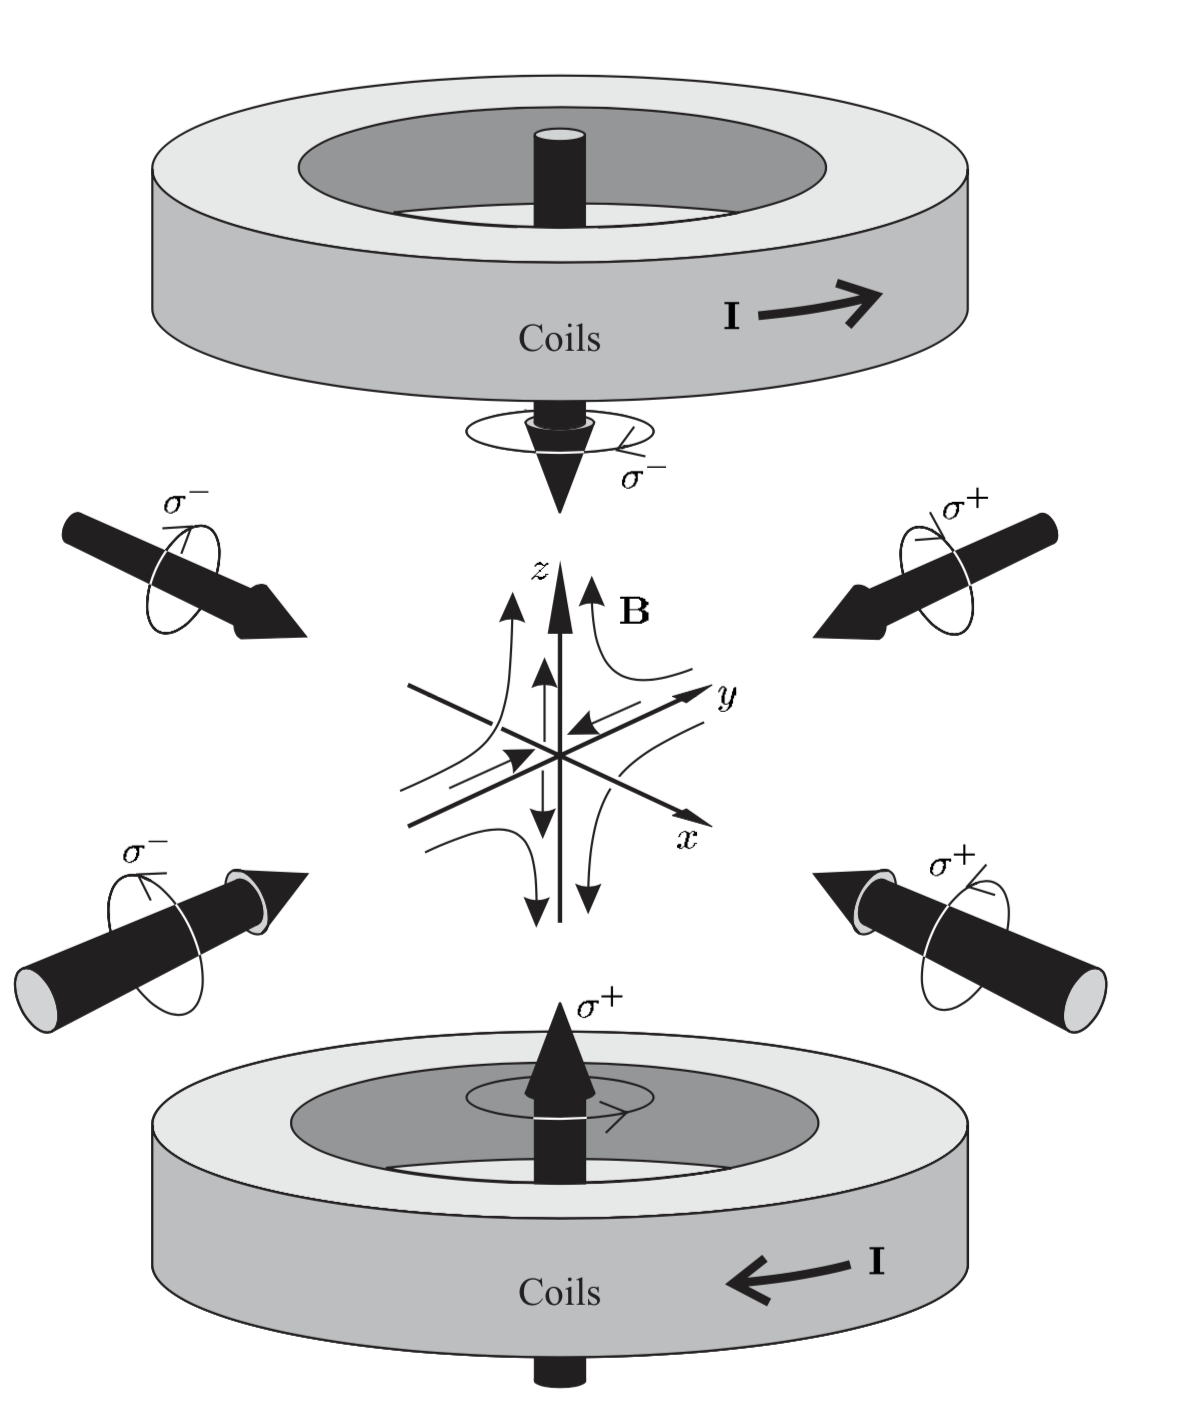
\includegraphics[width=40mm]{figures/MOT_circular_polarization.png}
\end{center}
 \caption{MOT}
 \label{MOT_circular_polarization}
\end{figure}

\begin{figure}[htbp]
 \begin{center}
  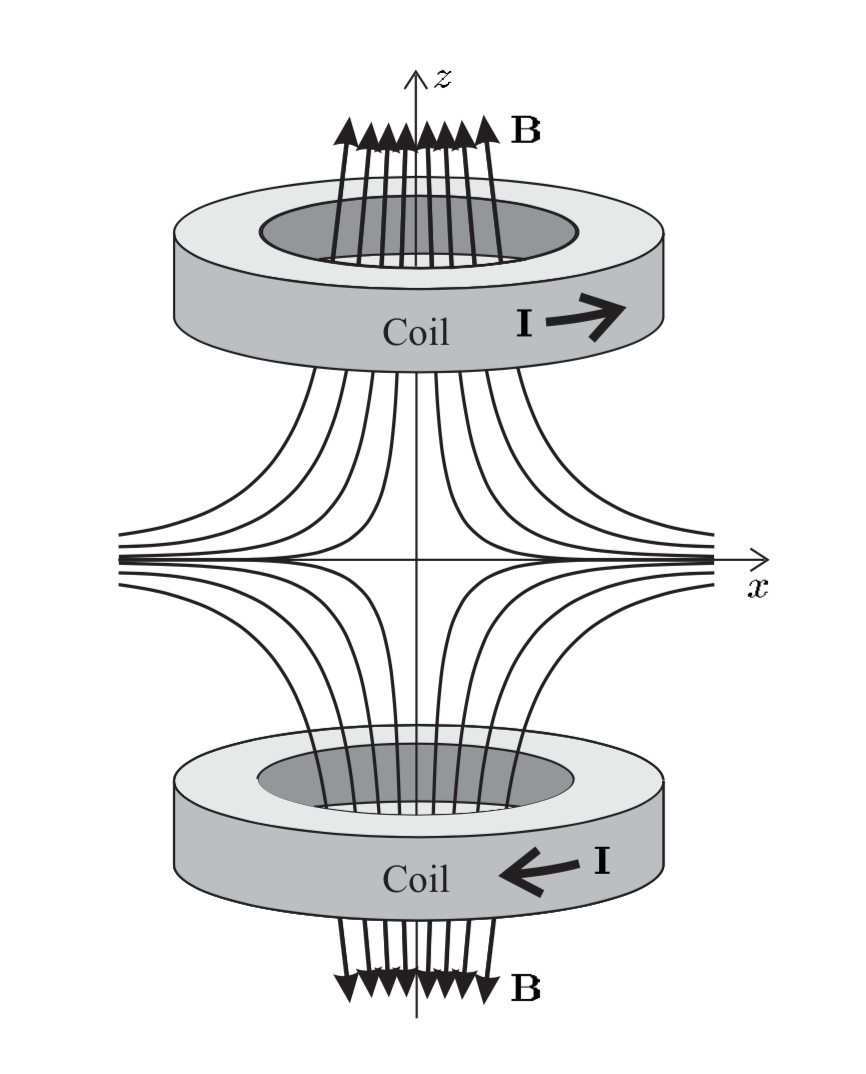
\includegraphics[width=50mm]{figures/MOT_magnetic_field.png}
\end{center}
 \caption{四重極磁場}
 \label{MOT_magnetic_field}
\end{figure}

\begin{figure}[htbp]
 \begin{center}
  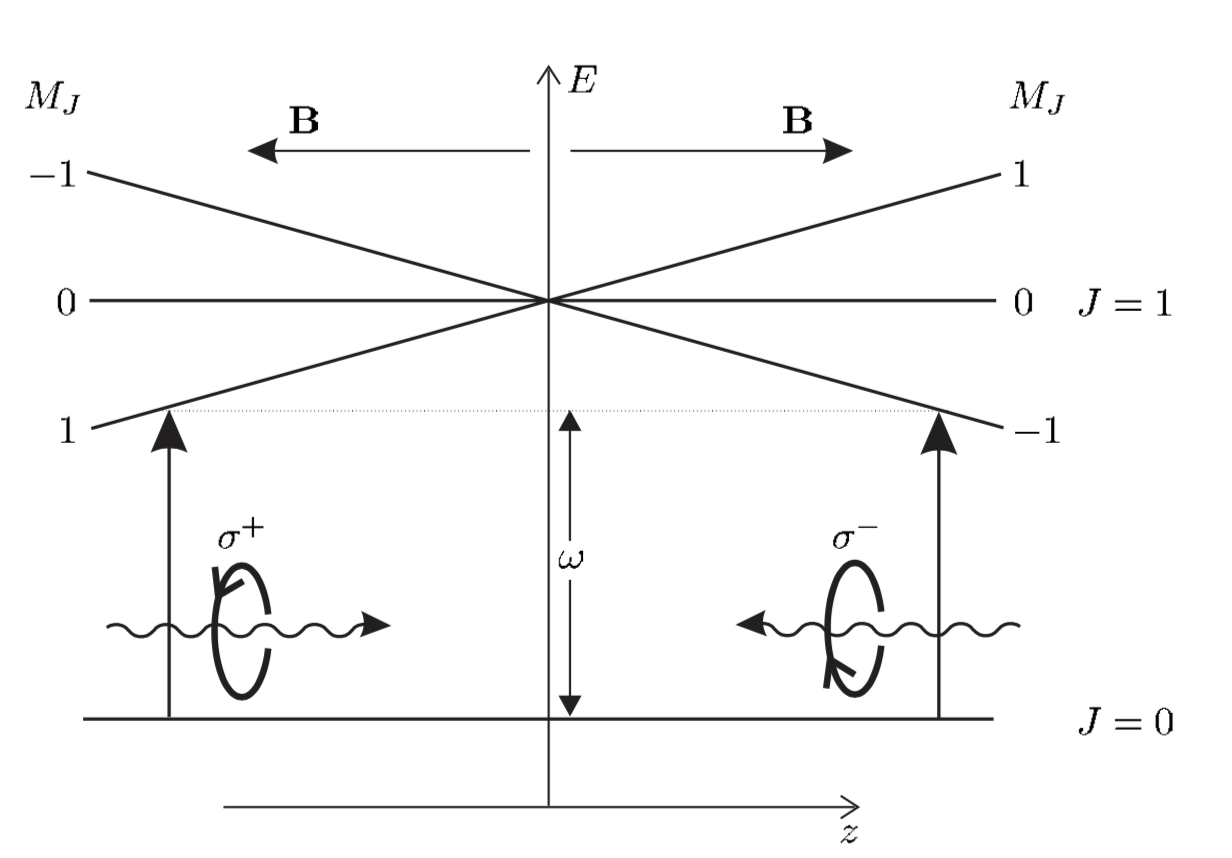
\includegraphics[width=50mm]{figures/MOT_zeeman_split.png}
 \end{center}
 \caption{四重極磁場によるゼーマン分裂}
 \label{MOT_zeeman_split}
\end{figure}
\end{comment}


\begin{figure}[htpb]
  \centering
    \begin{tabular}{c}

%----- MOTの構成 -----

      \begin{minipage}{0.50\hsize}
        \centering
          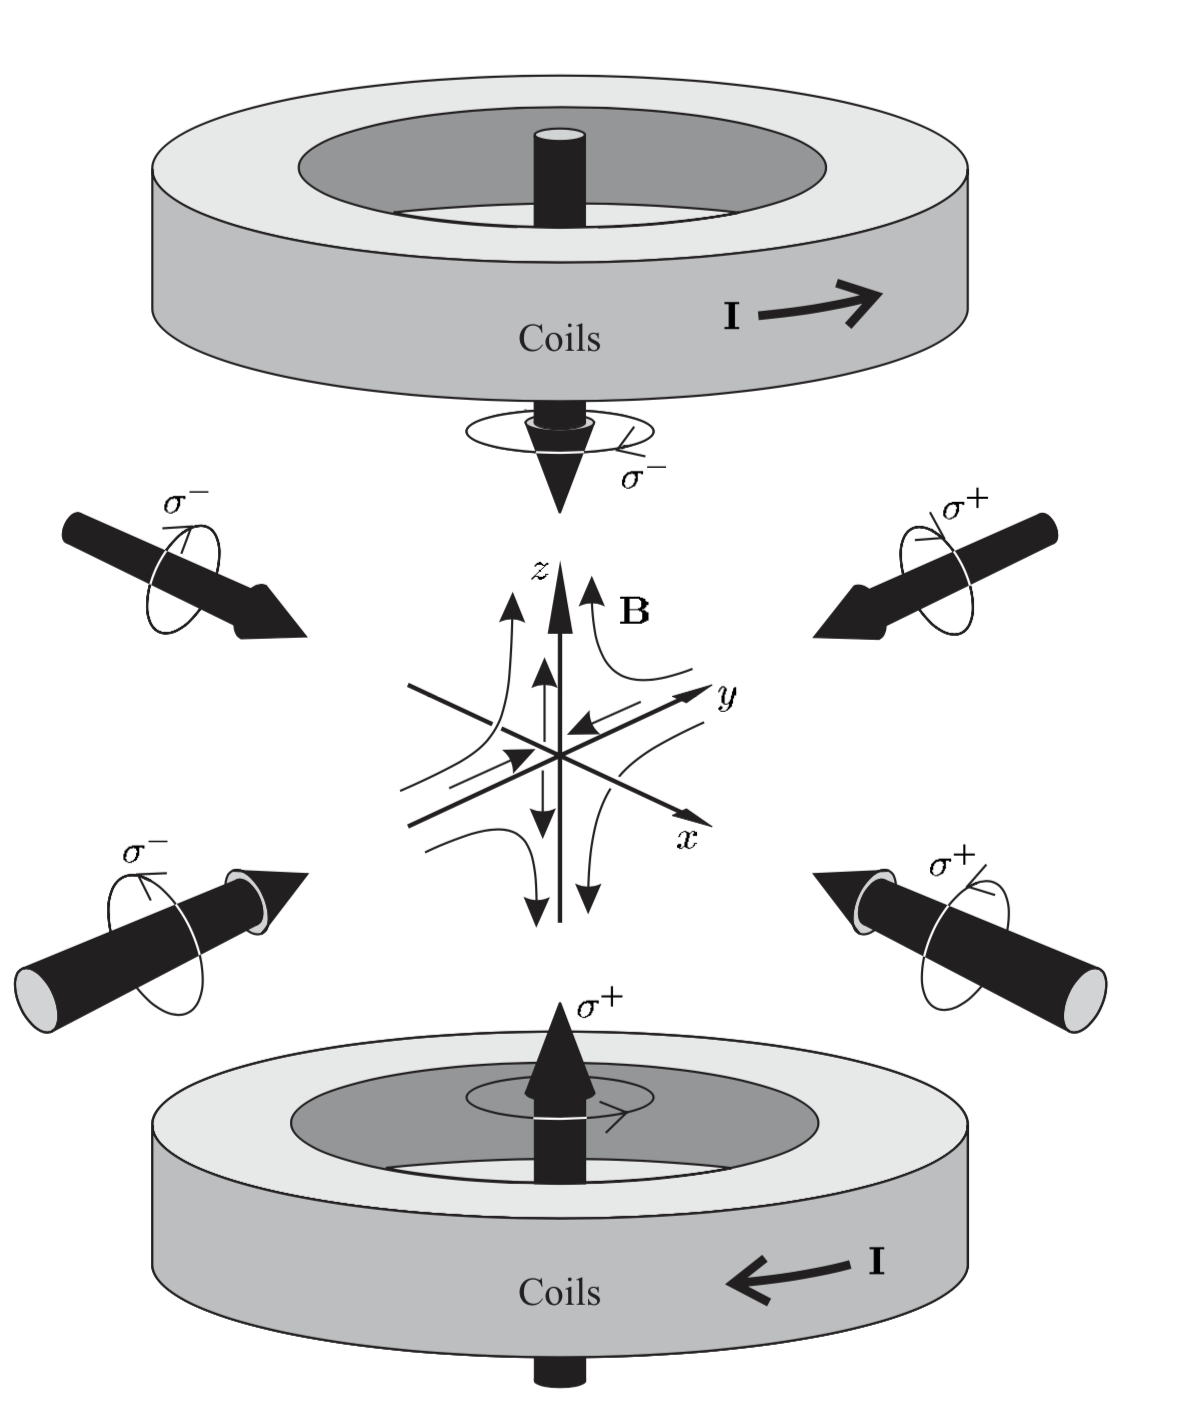
\includegraphics[keepaspectratio, scale=0.35, angle=0]
                          {figures/MOT_circular_polarization.png}
                          \caption{MOTの構成(文献\cite{Foot:1080846}より引用)}
                          \label{MOT_circular_polarization}
      \end{minipage}

%----- 四重極磁場 -----

      \begin{minipage}{0.50\hsize}
        \centering
          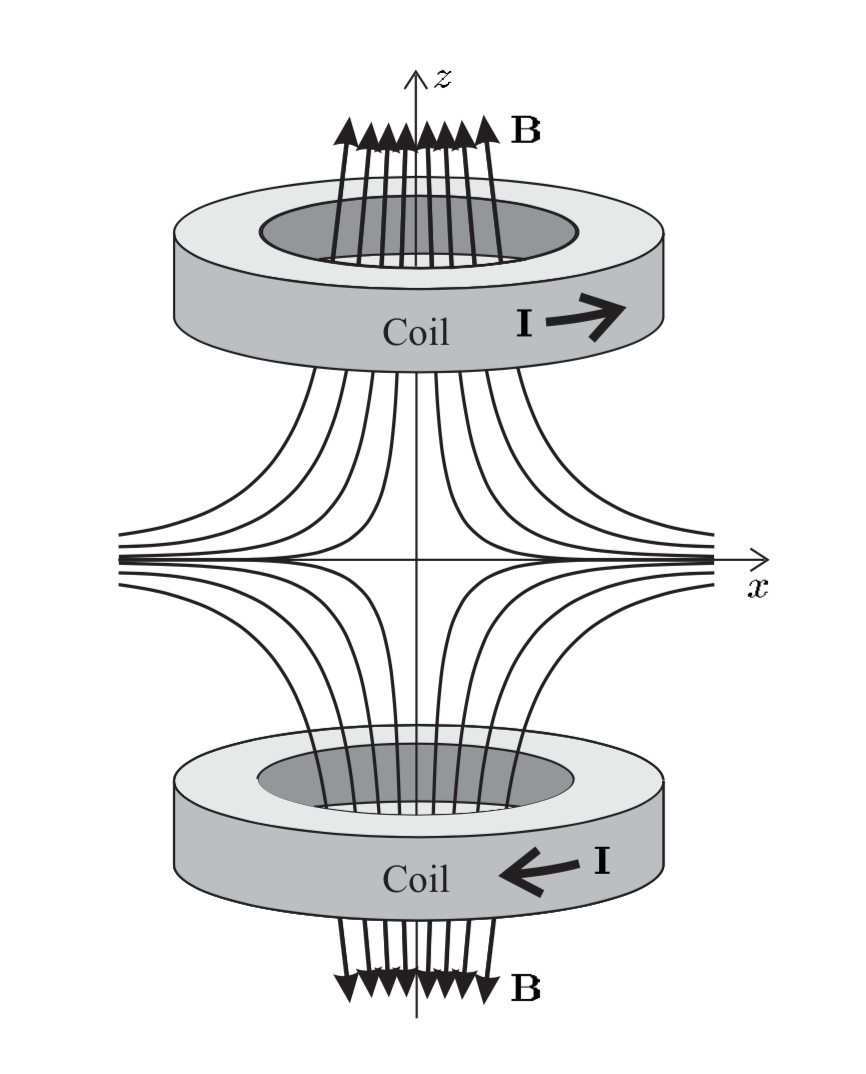
\includegraphics[keepaspectratio, scale=0.50, angle=0]
                          {figures/MOT_magnetic_field.png}
                          \caption{四重極磁場(文献\cite{Foot:1080846}より引用)}
                          \label{MOT_magnetic_field}
      \end{minipage} \\

%-----四重極磁場によるゼーマン分裂 -----

      \begin{minipage}{0.50\hsize}
        \centering
          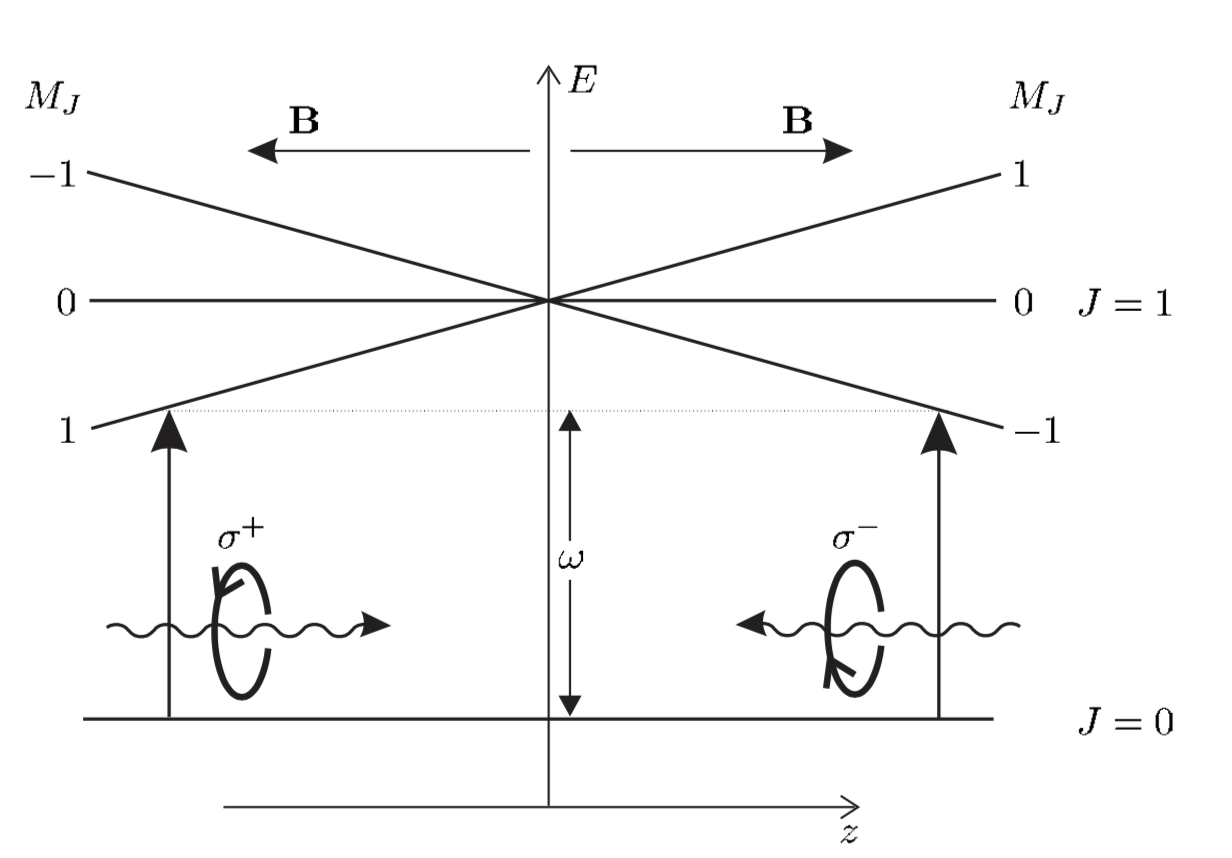
\includegraphics[keepaspectratio, scale=0.40, angle=0]
                          {figures/MOT_zeeman_split.png}
                          \caption{四重極磁場によるゼーマン分裂(文献\cite{Foot:1080846}より引用)}
                          \label{MOT_zeeman_split}
      \end{minipage}


    \end{tabular}
\end{figure}

\newpage
\section{飽和吸収分光法}
今回の実験ではMOTで使用する周波数のレーザーを得るために、「飽和吸収分光法」を利用している。通常の分光法では原子の遷移周波数の線幅は、温度に応じたドップラー拡がりを持っている。これに対し、飽和吸収分光法はドップラー拡がりを克服し、原子の遷移周波数を測定する手法である。\\右の図のように、レーザーをポンプ光とプローブ光に分けて原子の気体が入ったセルに照射し、プローブ光のセルの透過強度をを測定する。\\レーザーの周波数が原子の共鳴周波数$\omega_0$に合っているとき、セル通過後のプローブ光はポンプ光の影響を受けて、あまり原子に吸収されない。レーザーの周波数が$\omega_0$からずれている時はプローブ光の透過率はポンプ光からの影響を受けない。この効果により、レーザーの周波数を掃引すると、プローブ光の透過強度は右のようになる\cite{Foot:1080846}。

\section{光周波数コム}
\subsection{モード同期レーザーの概要}
モード同期レーザーは時間的に等間隔で出力されるパルス列である。このパルス列は共振器内の異なる縦モードの位相を同期することで得られる。モード同期の手法には能動的モード同期と受動的モード同期があるが、今回の実験では受動的モード同期を用いている。\\
 受動的モード同期法は共振器内に可飽和吸収体を設置することで行われる。これは強度が弱い光は吸収するが、高強度の光に対しては飽和を起こし高い透過率を示すような素子である。これによりパルスの裾では吸収が起こりパルスの頂点付近では吸収が起きないため、パルスの持続時間を短く保つことができる。このようにして、モード同期が自発的に行われる。\\
 レーザーの利得媒質としてチタニウムサファイア(Ti:Sa)を用いると、Ti:Sa自体が可飽和吸収体として振る舞う。これはTi:Sa中で起こるカーレンズ効果により、パルスの頂点付近の高強度の光は細くなりスリットを損失なく通過するが裾野の光はスリットで損失を受けるためTi:Saが実効的な可飽和吸収体として振る舞うためである。\\
 また、共振器内のミラーや利得媒質による群速度分散をプリズムやミラーで補償することで短パルスを維持する手法も用いられている。
\subsection{モード同期レーザーのスペクトル}
 モード同期レーザーの周波数領域でのスペクトルは等間隔のピークを持つ櫛状の形状となり、その周波数は
\begin{equation}
  f = nf_{rep} + f_{ceo}
\end{equation}
と表される\cite{Colloquium:Femtosecondopticalfrequencycombs}。ここで$f_{rep}$は繰り返し周波数、$f_{ceo}$はキャリア・エンベロープ・オフセット周波数と呼ばれる。このようなスペクトルの形状からモード同期レーザーは光周波数コムとも呼ばれる。\\
 また、$f_{ceo}$はパルス間の位相のシフトに対応しており、
 \begin{equation}
   f _ { 0 } = \frac { 1 } { 2 \pi } f _ { \mathrm { rep } } \Delta \phi _ { \mathrm { ce } }
 \end{equation}
と表される\cite{Colloquium:Femtosecondopticalfrequencycombs}。ここで、$\Delta \phi _ { \mathrm { ce } }$はパルス間の位相の変化を表す。このようなパルス間の位相の変化は、共振器内の分散による群速度と位相速度の差から生まれる。パルスは共振器内を一周する度に出力されるため、位相の変化は
\begin{equation}
  \Delta \phi _ { \mathrm { ce } } = \left( \frac { 1 } { \nu _ { g } } - \frac { 1 } { \nu _ { p } } \right) l _ { c } \omega _ { c }\ (\bmod 2 \pi)
\end{equation}
と表される\cite{Colloquium:Femtosecondopticalfrequencycombs}。ただし、$\nu _ { g }$、$\nu _ { p }$はそれぞれ群速度、位相速度を表し、$l_c$は共振器長、$\omega_c$はキャリア周波数を表す。
\section{テーパーアンプ}
\subsection{半導体の発光原理}
\subsection{テーパーアンプの構造}
(Tapered Amplifier, TA)

\chapter{過去の研究}
\section{従来の課題と光周波数コムによる冷却のメリット}

 従来のレーザー冷却では、アルカリ金属やアルカリ土類金属などの限られた原子しか冷却できなかった。この理由としては主に2つの理由が挙げられる。1つ目としては、水素や酸素を含む多くの原子の遷移エネルギーは真空紫外領域に相当しており現在はこの領域で十分な強度のレーザーを得ることができていないことがある。2つ目は、多くの原子ではエネルギー準位の構造が複雑であり励起された原子が準安定な準位に緩和してしまうので、これを励起するためのレーザーを用意する必要があり実験の系が複雑化してしまうことである\cite{PhysRevA.73.063407}。\\
 光周波数コムを用いた二光子のレーザー冷却は、2006年にKielpinski\cite{PhysRevA.73.063407}によって提案された。光周波数コムを用いることにより、上記の2つの課題を克服することができる。まず、光周波数コムは高強度のピークパワーをもつため、同じ時間平均パワーをもつcwレーザーに比べて高効率の非線形工学効果を利用することができ、より高強度の短波長のレーザーを得ることができる。また、光周波数コムの一つ一つのの縦モードがリポンプレーザーとして機能するために、実験の系を簡単にすることができる。これらの長所により、光周波数コムはcwレーザーよりも効率の良い二光子冷却を実現することができる\cite{PhysRevA.73.063407}。\\
 本章では、コムを用いた二光子冷却についての過去の研究の内容を紹介する。

\section{二光子コムによるレーザー冷却の理論}
 Jayichらの論文\cite{PhysRevX.6.041004}で説明されている、二光子遷移を用いたレーザー冷却の理論を紹介する。\\
コムによる二光子の遷移を考えるとき、パルスに含まれる二光子のエネルギーもまた、コム(櫛)を形成する。これを二光子コムと呼ぶことにすると、二光子コムのn番目の縦モードの周波数は
\begin{equation}
f_n = nf_r + 2f_0
\end{equation}
となる。ただし、$f_r$:は繰り返し周波数、$f_0$はキャリアエンベロープオフセット周波数を表す。チャープのモード同期レーザーについては実効的な共鳴ラビ周波数を求めることができる。二光子コムのn番目のコムの歯共鳴ラビ周波数は、
\begin{equation}
\Omega _{n}=\sum _{p}\frac {g^{\left( 1\right) }_{p}g^{\left( 2\right) }_{n-p}}{2\Delta p}
\end{equation}\\
ただし、$g^{\left( 1\right) }_{p}$は$p$番目のコムの歯による基底状態から中間状態への共鳴一光子ラビ周波数、$g^{\left( 2\right) }_{p}$は$p$番目のコムの歯による中間状態から励起状態への共鳴一光子ラビ周波数を表す。
$\Delta _{p}=pf_{r}+f_{0}-f_{gi}$は一光子の中間状態からの離調である。ただし、$f_{gi}$は基底状態から中間状態へのエネルギー差をプランク定数$h$で割ったものである。\\
二光子コムのN番目のコムの歯が共鳴周波数に最も近いとき、速度$v$で動く原子の励起確率の時間平均は、
\begin{equation}
\gamma_{comb} = \frac{\Omega^2_{N}T_r} {4} \frac{\sinh(\gamma T_r/2)}{\cosh(\gamma T_r/2) - \cos(\delta_N(\bm{v})T_r)}
\end{equation}
ここで、$\delta _{N}\left( v\right) \equiv 2\pi ( f_{\mu }-f_{ge}-f_{N}\widehat {\bm{k}}\cdot {\bm{v}}/c )$は$N$番目の二光子コムの歯の共鳴周波数からの離調を表す。$f_{ge}$は励起状態と基底状態のエネルギー差をプランク定数で割ったもの、$\widehat {\bm{k}}$はレーザーの進行方向の単位ベクトル、$\gamma$は励起準位の自然幅を表す。\\
離調$\delta _{N}\left( v\right)$と自然幅$\gamma$の両方がコムの歯の間隔($2\pi f_r$)よりも小さいとき、二光子コムは二光子ラビ周波数$\Omega_N$の一つの縦モードとして扱うことができる。この近似の下では、励起確率は
\begin{equation}
\gamma_N = \frac{\Omega^2_N}{\gamma}\frac{1}{1 + [2\delta_N(\bm{v})/\gamma]^2}
\end{equation}
と表せる。\\
 また、(二色のコムによる冷却ではなく)縮退したコムによる二光子冷却の場合、ドップラー冷却限界温度は
\begin{equation}
  T_D = \frac{3}{4}\frac{\hbar\gamma}{2k_B}
\end{equation}
となることが分かっている。($k_B$はボルツマン定数)

\section{二光子コムによる冷却の実証}
 Jayichらの論文\cite{PhysRevX.6.041004}で初めて光周波数コムを用いた二光子冷却の実証実験が行われた。Jaychらのグループはルビジウムの縮退した二光子のコムによる一次元のレーザー冷却に成功し、57 $\mu$ Kを達成している。



\chapter{テープアンプを用いたモード同期レーザーの構築}
\section{テープアンプのマウンターの組み立て}
\section{光学系の組み立て}

\newpage
\chapter{二色の光周波数コムによる二光子冷却}

\chapter{考察}
\chapter{まとめと展望}






\bibliography{reference}
\end{document}
